\documentclass[14pt]{extbook}
\usepackage{multicol, enumerate, enumitem, hyperref, color, soul, setspace, parskip, fancyhdr} %General Packages
\usepackage{amssymb, amsthm, amsmath, bbm, latexsym, units, mathtools} %Math Packages
\everymath{\displaystyle} %All math in Display Style
% Packages with additional options
\usepackage[headsep=0.5cm,headheight=12pt, left=1 in,right= 1 in,top= 1 in,bottom= 1 in]{geometry}
\usepackage[usenames,dvipsnames]{xcolor}
\usepackage{dashrule}  % Package to use the command below to create lines between items
\newcommand{\litem}[1]{\item#1\hspace*{-1cm}\rule{\textwidth}{0.4pt}}
\pagestyle{fancy}
\lhead{Progress Quiz 4}
\chead{}
\rhead{Version C}
\lfoot{9187-5854}
\cfoot{}
\rfoot{Spring 2021}
\begin{document}

\begin{enumerate}
\litem{
Solve the radical equation below. Then, choose the interval(s) that the solution(s) belongs to.\[ \sqrt{40 x^2 - 12} - \sqrt{-4 x} = 0 \]\begin{enumerate}[label=\Alph*.]
\item \( x_1 \in [0.08, 1.17] \text{ and } x_2 \in [0.52,0.67] \)
\item \( x_1 \in [-0.9, -0.24] \text{ and } x_2 \in [0.42,0.53] \)
\item \( \text{All solutions lead to invalid or complex values in the equation.} \)
\item \( x \in [-0.9,-0.24] \)
\item \( x \in [0.08,1.17] \)

\end{enumerate} }
\litem{
Solve the radical equation below. Then, choose the interval(s) that the solution(s) belongs to.\[ \sqrt{81 x^2 + 35} - \sqrt{108 x} = 0 \]\begin{enumerate}[label=\Alph*.]
\item \( x_1 \in [-0.82, -0.56] \text{ and } x_2 \in [-1.4,-0.5] \)
\item \( \text{All solutions lead to invalid or complex values in the equation.} \)
\item \( x \in [0.14,0.57] \)
\item \( x \in [0.58,1] \)
\item \( x_1 \in [0.14, 0.57] \text{ and } x_2 \in [0.6,0.9] \)

\end{enumerate} }
\litem{
Choose the graph of the equation below.\[ f(x) = \sqrt[3]{x + 12} - 7 \]\begin{enumerate}[label=\Alph*.]
\begin{multicols}{2}\item 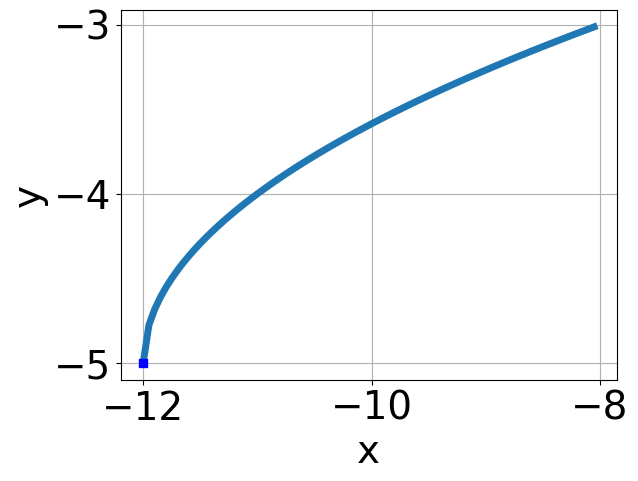
\includegraphics[width = 0.3\textwidth]{../Figures/radicalEquationToGraphAC.png}\item 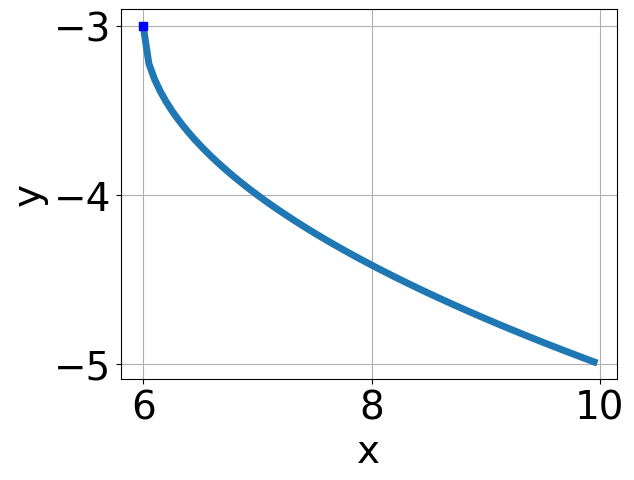
\includegraphics[width = 0.3\textwidth]{../Figures/radicalEquationToGraphBC.png}\item 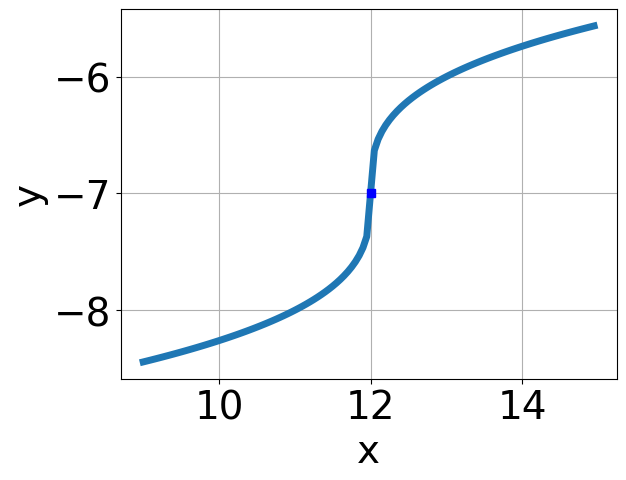
\includegraphics[width = 0.3\textwidth]{../Figures/radicalEquationToGraphCC.png}\item 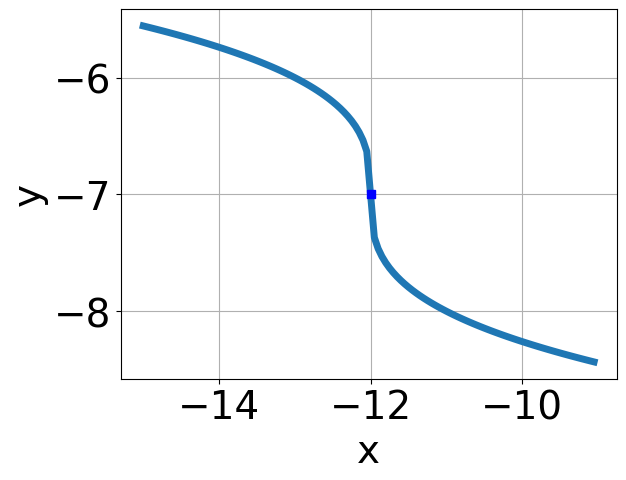
\includegraphics[width = 0.3\textwidth]{../Figures/radicalEquationToGraphDC.png}\end{multicols}\item None of the above.
\end{enumerate} }
\litem{
What is the domain of the function below?\[ f(x) = \sqrt[5]{6 x + 4} \]\begin{enumerate}[label=\Alph*.]
\item \( (-\infty, \infty) \)
\item \( \text{The domain is } [a, \infty), \text{   where } a \in [-0.81, -0.48] \)
\item \( \text{The domain is } (-\infty, a], \text{   where } a \in [-2, -0.7] \)
\item \( \text{The domain is } [a, \infty), \text{   where } a \in [-1.61, -1.01] \)
\item \( \text{The domain is } (-\infty, a], \text{   where } a \in [-1.2, 1] \)

\end{enumerate} }
\litem{
Choose the equation of the function graphed below.
\begin{center}
    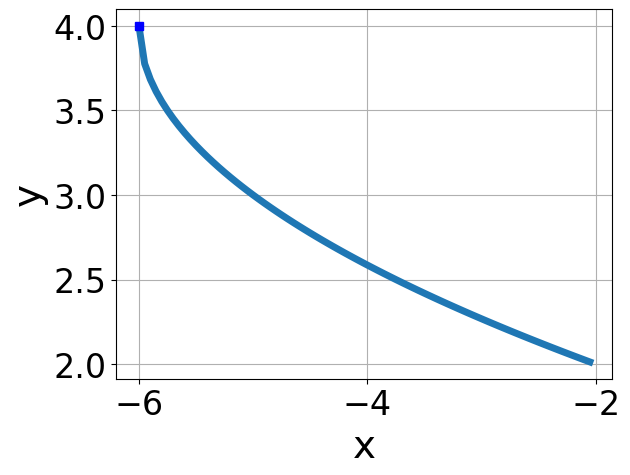
\includegraphics[width=0.5\textwidth]{../Figures/radicalGraphToEquationCopyC.png}
\end{center}
\begin{enumerate}[label=\Alph*.]
\item \( f(x) = - \sqrt[3]{x + 14} + 3 \)
\item \( f(x) = - \sqrt[3]{x - 14} + 3 \)
\item \( f(x) = \sqrt[3]{x - 14} + 3 \)
\item \( f(x) = \sqrt[3]{x + 14} + 3 \)
\item \( \text{None of the above} \)

\end{enumerate} }
\litem{
What is the domain of the function below?\[ f(x) = \sqrt[4]{-3 x + 4} \]\begin{enumerate}[label=\Alph*.]
\item \( (-\infty, a], \text{where } a \in [0.14, 1.27] \)
\item \( [a, \infty), \text{where } a \in [-0.9, 1] \)
\item \( (-\infty, \infty) \)
\item \( (-\infty, a], \text{ where } a \in [1.18, 2.02] \)
\item \( [a, \infty), \text{where } a \in [1.1, 2.4] \)

\end{enumerate} }
\litem{
Choose the equation of the function graphed below.
\begin{center}
    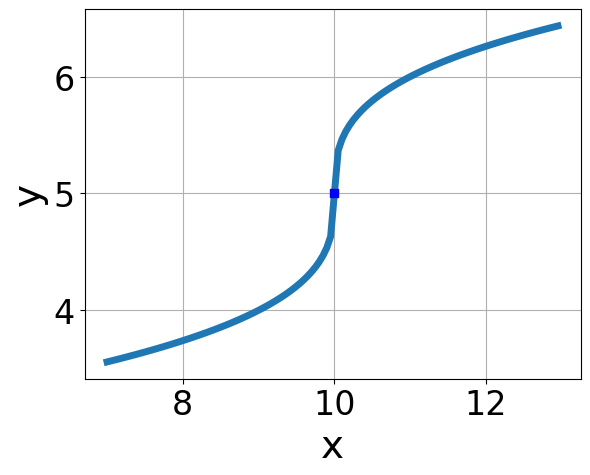
\includegraphics[width=0.5\textwidth]{../Figures/radicalGraphToEquationC.png}
\end{center}
\begin{enumerate}[label=\Alph*.]
\item \( f(x) = - \sqrt[3]{x + 6} - 6 \)
\item \( f(x) = \sqrt[3]{x - 6} - 6 \)
\item \( f(x) = \sqrt[3]{x + 6} - 6 \)
\item \( f(x) = - \sqrt[3]{x - 6} - 6 \)
\item \( \text{None of the above} \)

\end{enumerate} }
\litem{
Choose the graph of the equation below.\[ f(x) = \sqrt{x - 8} + 4 \]\begin{enumerate}[label=\Alph*.]
\begin{multicols}{2}\item 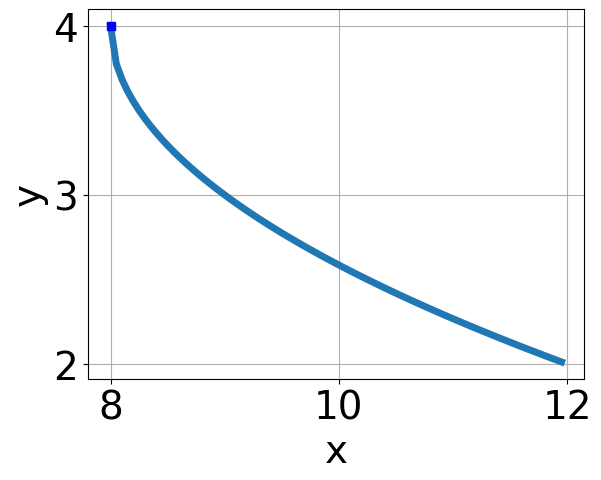
\includegraphics[width = 0.3\textwidth]{../Figures/radicalEquationToGraphCopyAC.png}\item 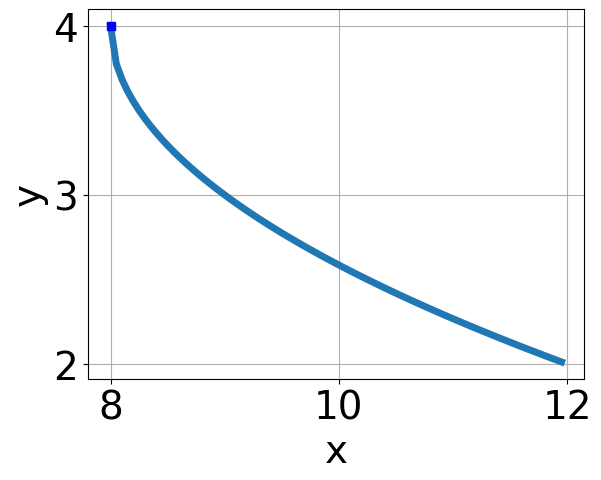
\includegraphics[width = 0.3\textwidth]{../Figures/radicalEquationToGraphCopyBC.png}\item 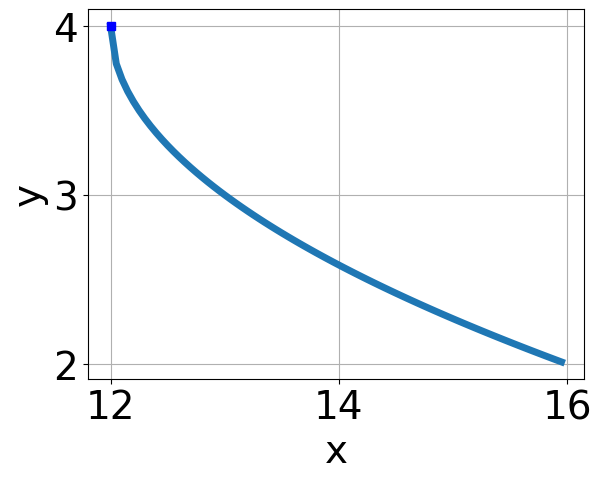
\includegraphics[width = 0.3\textwidth]{../Figures/radicalEquationToGraphCopyCC.png}\item 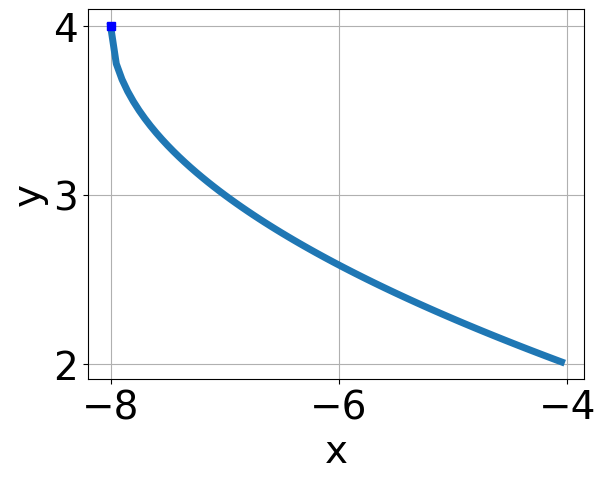
\includegraphics[width = 0.3\textwidth]{../Figures/radicalEquationToGraphCopyDC.png}\end{multicols}\item None of the above.
\end{enumerate} }
\litem{
Solve the radical equation below. Then, choose the interval(s) that the solution(s) belongs to.\[ \sqrt{-6 x - 9} - \sqrt{4 x - 9} = 0 \]\begin{enumerate}[label=\Alph*.]
\item \( \text{All solutions lead to invalid or complex values in the equation.} \)
\item \( x \in [-2.04,-1.8] \)
\item \( x \in [-0.76,0] \)
\item \( x_1 \in [-1.57, -1.39] \text{ and } x_2 \in [1.25,6.25] \)
\item \( x_1 \in [-1.57, -1.39] \text{ and } x_2 \in [-2,1] \)

\end{enumerate} }
\litem{
Solve the radical equation below. Then, choose the interval(s) that the solution(s) belongs to.\[ \sqrt{4 x - 8} - \sqrt{-5 x - 5} = 0 \]\begin{enumerate}[label=\Alph*.]
\item \( x_1 \in [0.02, 0.8] \text{ and } x_2 \in [1,8] \)
\item \( x_1 \in [-1.15, -0.45] \text{ and } x_2 \in [1,8] \)
\item \( x \in [0.4,2.72] \)
\item \( \text{All solutions lead to invalid or complex values in the equation.} \)
\item \( x \in [0.02,0.8] \)

\end{enumerate} }
\end{enumerate}

\end{document}